\documentclass{beamer}

\mode<presentation>
{
  \useinnertheme[shadow=true]{rounded} % default from Warsaw theme
  \useoutertheme[subsection=false]{miniframes}

  \usecolortheme{orchid} % default from Warsaw theme
  \usecolortheme{whale} % default from Warsaw theme
  \usecolortheme{beaver} % this overrides both orchid and whale, as far as I see, but keep them for safety

  % these override \usecolortheme above
  \setbeamercolor{frametitle}{bg=,fg=darkred!80!black}
  \setbeamercolor{frametitle right}{bg=}
  \setbeamercolor{palette tertiary}{fg=black,bg=gray!15!white}

  \usefonttheme[onlylarge]{structurebold}
  \setbeamerfont{block title}{size={}} % default from Warsaw theme
  \setbeamerfont{frametitle}{series=\bfseries} % probably taken care of by structurebold anyway, but keep in case useful for the future

  \setbeamercovered{transparent}
}

\usepackage[polish]{babel}
\usepackage[utf8]{inputenc}
\usepackage{times}
\usepackage[T1]{fontenc}

\title{Komponowanie shaderów w X3D}

\author[Michalis Kamburelis]{Michalis Kamburelis \\ \texttt{michalis.kambi@gmail.com}}


\AtBeginSection[]
{
  \begin{frame}<beamer>{Outline}
    \tableofcontents[currentsection,currentsubsection]
  \end{frame}
}

\begin{document}

{
  % logo on title page
  \pgfdeclareimage[height=2cm]{ii-and-kambivrml}{ii-and-kambivrml}
  \logo{\pgfuseimage{ii-and-kambivrml}}
  \begin{frame}
    \titlepage
  \end{frame}
}

\begin{frame}{Outline}
  \tableofcontents
  % You might wish to add the option [pausesections]
\end{frame}

\section{Wstęp}

\begin{frame}{Wstęp}
Pokazaliśmy jak elegancko i łatwo tworzyć i łączyć efekty graficzne
oparte na shaderach.

\begin{itemize}
  \item Rozszerzenie dwóch zintegrowanych ze sobą języków (X3D i GLSL).
  \item Faktycznie wykonalne (działająca implementacja i przykłady w ~miesiąc).
\end{itemize}

Proste, ale nikt inny tego jeszcze nie zrobił :)

\begin{itemize}
  \item Przynajmniej nie bez wymyślania zupełnie nowego języka pisania shaderów
    (AnySL, Spark, Sh). Ale nowe języki nie zdobywają popularności,
    bo zazwyczaj wymagają przepisania całego renderowania.
    Nasz pomysł to eleganckie rozszerzenie GLSL  i X3D.
    % glsl - (który jest podstawą OpenGL, więc znają go wszyscy
  \item Wyniki bardzo obiecujące. Będą ładne obrazki.
    Różne (poprzednio nietrywialnych) algorytmy na shaderach stają się
    trywialne.
    % Istotnie pozwalam na programowanie i łączenie efektów
    % za pomocą shaderów w bardzo wygodny sposób.
    %  IMHO dopiero teraz GLSL jest użyteczny dla autorów.
\end{itemize}
\end{frame}

\section{Co to jest X3D, co to są shadery}

\begin{frame}[fragile]{X3D}

\begin{itemize}
  \item X3D to język do opisu światów 3D.
  \item Otwarty, popularny standard.
  \item Proste rzeczy są proste.
  \item Drzewo węzłów w prostych przypadkach (de facto, skierowany graf
    --- mogą być cykle).
  \item Każdy węzeł ma pola i dzieci.
\end{itemize}

\begin{exampleblock}{Przykład}
\begin{semiverbatim}
\#X3D V3.2 utf8
PROFILE Interchange
Shape \{
  geometry Sphere \{ radius 2 \}
\}
\end{semiverbatim}
\end{exampleblock}
\end{frame}

\begin{frame}[fragile]{X3D - przykład XML}

\begin{exampleblock}{Alternatywna wersja poprzedniego przykładu}
\begin{semiverbatim}
...
<X3D version="3.2" profile="Interchange" ...>
  <Scene>
    <Shape>
      <Sphere radius="2" />
    </Shape>
  </Scene>
</X3D>
\end{semiverbatim}
\end{exampleblock}

\end{frame}

\begin{frame}{X3D jako język programowania}

Kilka ciekawostek które czynią X3D bardziej interesującym:

\begin{itemize}
  \item DEF/USE: referencje, dla wszystkich węzłów.
  \item Mechanizm zdarzeń: wysyłanie i reagowane na zdarzenia.
    Deklaratywny odpowiednik wywołania metody obiektu.
    Np. otwórz drzwi kiedy user kliknie na klamkę.
  \item Prototypy: można definiować nowe, pełnowartościowe,
    węzły jako kombinację istniejących.
  \item Ogólnie "format modeli 3D" to prosta definicja dla użytkowników.
    Definicja dla nas to "całkiem ładny deklaratywny język programowania",
    który akurat ma mnóstwo wbudowanych węzłów na grafiki 3D.
  \item Script: integracja z innymi językami (np. JavaScript) naturalnie łatwa.
     %  np. JavaScript. U mnie --- z własnym prostym językiem skryptowym
     % oraz ze skompilowanym kodem w ObjectPascalu.
     % Więcej nowinek w vrml\_engine\_doc, sekcja "advanced features".
\end{itemize}
\end{frame}

\begin{frame}{Shadery}
Shadery:
\begin{itemize}
  \item Języki do cieniowania obiektów 3D. Uproszczenie: zrób coś per-vertex,
    rasteryzuj, zrób coś per-pixel.
    % Chociaż przy pomocy pewnych sztuczek (tekstury oparte na float,
    % render to textury) można je wykorzystać do ogólnych obliczeń,
    % obecnie do ogólnych obliczeń wygodniejsze są CUDA/OpenCL
    % (google.com/q=gpgpu).
    % Można próbować
    % geom shader
  \item Nas interesują shadery na GPU, czyli do renderowania w czasie
    rzeczywistym. GLSL (OpenGL), Cg (NVidia -> OpenGL lub Direct 3D),
    HLSL (Direct 3D).
  \item Naturalnie, X3D posiada węzły do definiowania shaderów.
\end{itemize}
\end{frame}

\begin{frame}[fragile]{Shadery w X3D - przykład}
\begin{exampleblock}{Przykład X3D + GLSL}
\begin{semiverbatim}
\#X3D V3.2 utf8
PROFILE Interchange
Shape \{
  appearance Appearance \{ shaders ComposedShader \{
    language "GLSL"
    parts [
      ShaderPart \{ type "FRAGMENT"
        url "data:text/plain,
        \textbf{void main(void)}
        \textbf{\{}
          \textbf{gl\_FragColor = vec4(1.0, 0.0, 0.0, 1.0);}
        \textbf{\}}" \}
    ]
  \} \}
  geometry Sphere \{ radius 2 \}
\}
\end{semiverbatim}
\end{exampleblock}
\end{frame}

\begin{frame}{O shaderach w X3D}

Co złego, co dobrego w shaderach w X3D?

\begin{itemize}
  \item + Wybierz pierwszy obsługiwany shader.
  \item + Można łatwo przekazać do shadera wartości uniform (per-object)
    albo attribute (per-vertex).\\
    Np. przekaż aktualny czas (\texttt{TimeSensor.time} w X3D) to shadera trywialnie.
  \item Shader zastępuje domyślne obliczenia:
    \begin{itemize}
      \item + Łatwe do implementacji, bo właśnie tak działa GPU, na to pozwala
        OpenGL etc.
      \item - \textbf{Trudne} implementowanie własnych shaderów.
        Zanim zaczniesz pisać swój efekt, najpierw odtwórz algorytm
        standardowego renderowania. Głupie, bo renderer umie go wygenerować.
        Możesz go skopiować i zorientować się gdzie dodać kod, ale...
      \item - \textbf{Powstają shadery 1-razowego użytku}.
        Konkretny kod shadera przywiązuje Cię do wielu ustawień sceny
        (ile, jakie tekstury, światła etc.).
        Ogólny shader (uwzględniający wszystkie możliwości) nie jest możliwy,
        bo nie ma szans działać w rozsądnycm czasie.
      \item - \textbf{Wszystkie efekty w jednym worku}.
        Usuwanie / dodawanie efektu oznacza wstawianie kodu do istniejącego
        dużego shadera.
    \end{itemize}
\end{itemize}
\end{frame}

\section{Nasz pomysł}

\begin{frame}{Dlaczego}
Chcelibyśmy intensywnie używać shaderów. Każda właściwość 3D powinna
być programowalna --- po to stworzono shadery.

Ale tradycyjne podejscie, ,,napisz shader który robi wszystko'',
uniemożliwia to. Zaprogramowanie najmniejszej zmiany (np. przefiltruj
światło przez szablon) wymaga reimplementacji skomplikowanego algorytmu naokoło.
\end{frame}

\begin{frame}{Rozwiązanie}
Pozwól programować efekty które modyfikują istniejące zachowanie.

% TODO: ramka, cos jak do twierdzenia
\textbf{Idea 1}: bardzo prosty w użyciu mechanizm do definiowania nowych,
i używania istniejących, ,,gniazd'' (plugs) --- miejsc gdzie można
dodać własne obliczenia. Żeby użyć gniazda o nazwie \texttt{texture\_apply},
po prostu zdefiniuj funkcję o magicznej nazwie \texttt{PLUG\_texture\_apply},
i użyj nowego węzła \texttt{Effect}.

\begin{itemize}
  \item + Zachowujemy pełną siłę języka shaderów (GLSL w naszej implementacji).
    %% - You still have the full power of shading language like GLSL
    %%   (we do not hide it from you, we do not invent any new language
    %%   for writing shaders, and implementation doesn't have to do any
    %%   difficult operations to process your shading language code).
  \item + Implementacja w rendererze łatwa: rozszerzamy istniejący język).
  \item + Implementacja efektów łatwa: zaczynamy od razu pisać nasz algorytm,
    wskazujemy tylko gdzie go wstawić.
  \item + Efekty reusable: wstawiane w wewnętrzny shader, wygenerowany
    znając tekstury, oświetlenie etc.
  \item + Efekty można łączyć: wiele efektów może używać tych samych gniazd.
\end{itemize}
\end{frame}

\begin{frame}{Wewnętrzne efekty}

Rozwiązanie przydatne także do wewnętrznych efektów.

\begin{itemize}
  \item Shadow maps: filtruj odpowiednie źródło światła,
  \item Bump mapping klasyczny: zmien wektor normalny na podstawie tekstury,
  \item Mgła: wymieszaj końcowy kolor pixela z kolorem mgły.
\end{itemize}

\begin{figure}
  \centering
  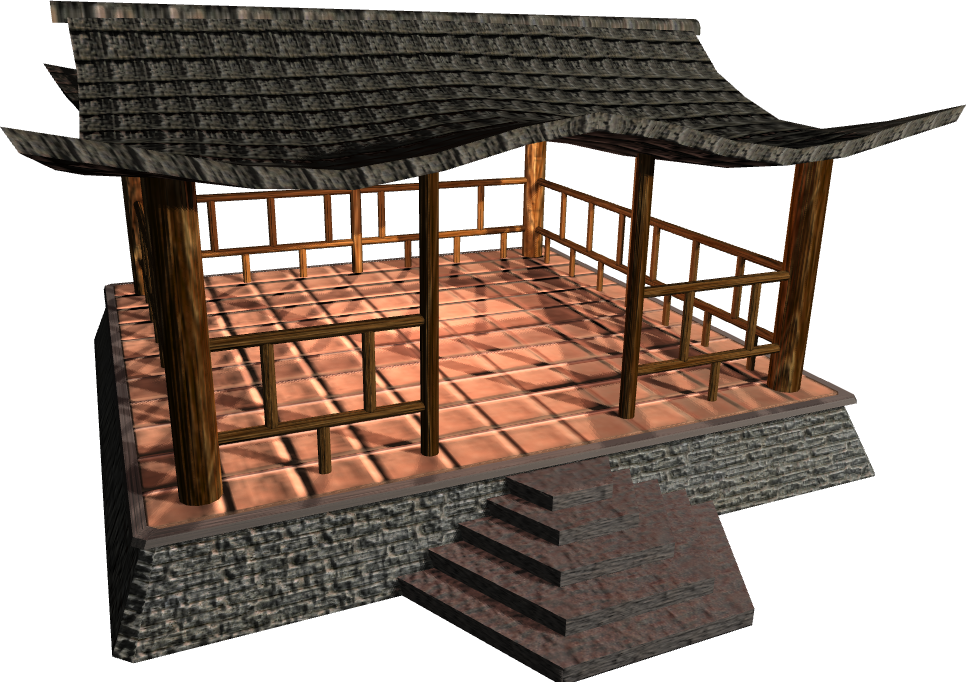
\includegraphics[width=1.8in]{../rhan_shrine_5_everything}
  \caption{Połączenie dwóch shadow maps i bump mapping}
\end{figure}
\end{frame}

\begin{frame}[fragile]{Przykład}
\begin{exampleblock}{Przykład naszych efektów}
\begin{semiverbatim}
# Poniższe należy włożyć do środka Appearance
# z poprzednich przykładów
effects Effect \{
  language "GLSL"
  parts EffectPart \{
    type "FRAGMENT"
    url "data:text/plain,
\textbf{    void PLUG\_texture\_apply(}
\textbf{      inout vec4 fragment\_color,}
\textbf{      const in vec3 normal)}
\textbf{    \{}
\textbf{      fragment\_color.rgb *= 2.0;}
\textbf{    \}}"
  \}
\}
\end{semiverbatim}
\end{exampleblock}
\end{frame}

\begin{frame}{Szczegóły}
\begin{itemize}
  \item Nowy węzeł \texttt{Effect}: wybierz język shaderów.
  \item Nowy węzeł \texttt{EffectPart}: wybierz typ (vertex, pixel, etc.).
  \item Można definiować własne uniform w \texttt{Effect}, np. przekazać
    teksturę albo czas do efektu.
    % jak ComposedShader
  \item Wszystkie efekty będą dodane do bazowego shadera. (Upraszczając.)
  \item Stary \texttt{ComposedShader} modyfikuje bazowy shader.
    W ten sposób stary \texttt{ComposedShader} też jest lepszy:
    może współpracować z wewnętrznymi efektami (shadow maps),
    i efektami użytkownika (z węzłów \texttt{Effect}).
\end{itemize}
\end{frame}

\begin{frame}{Przykład łączenia: fresnel\_and\_toon}
\begin{figure}
  \centering
  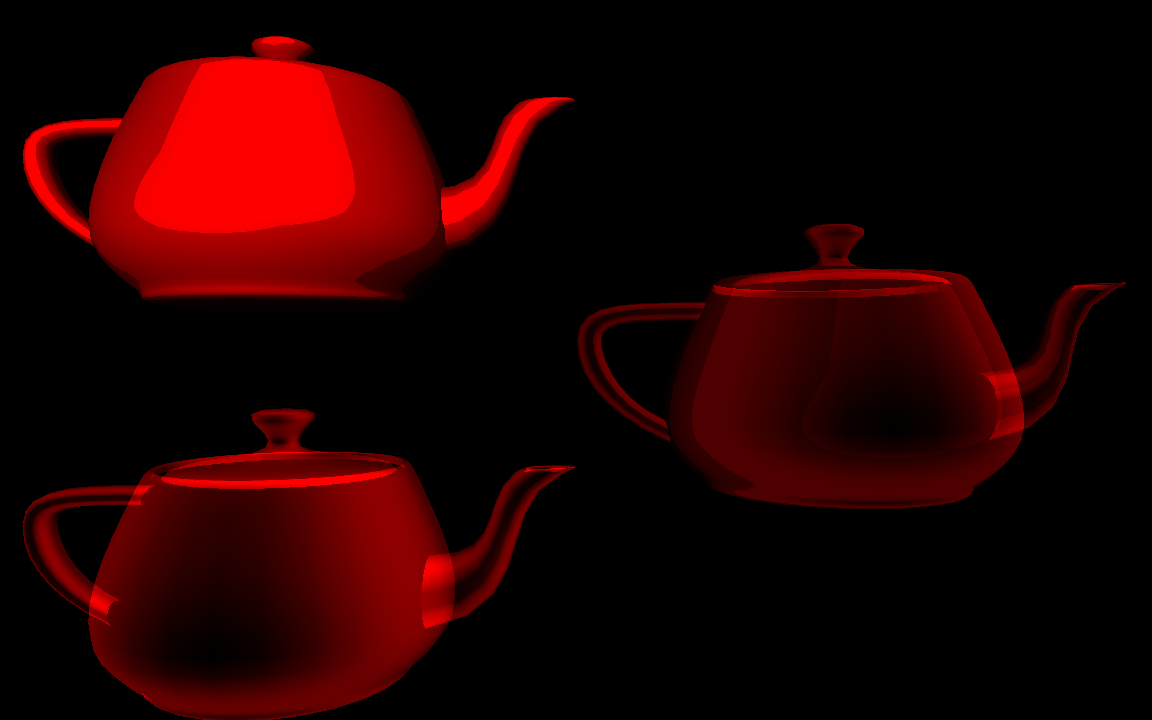
\includegraphics[width=1.8in]{../fresnel_and_toon}
  \caption{Połączenie dwóch prostych efektów Fresnela i cieniowania kreskówkowego}
\end{figure}

(Kod: \texttt{demo\_models/compositing\_shaders/fresnel\_and\_toon.x3dv})

  %% : show the X3D source:
  %%   I can just say: "this is a list of effects you should use:
  %%   this one, and this one. Now make it happen."
  %%   And both effects are applied.
\end{frame}

\begin{frame}{Efekty dla źródeł światła}
Idea 2: efekty można dodawać nie tylko do widocznych obiektów 3D,
także do innych elementów sceny. W ten sposob można zdefiniować
światło które ma specyficzny kształt, specyficznie równanie etc.

Takie światło automatycznie współpracuje z cieniami, bump mapping etc.!

\begin{figure}
  \centering
  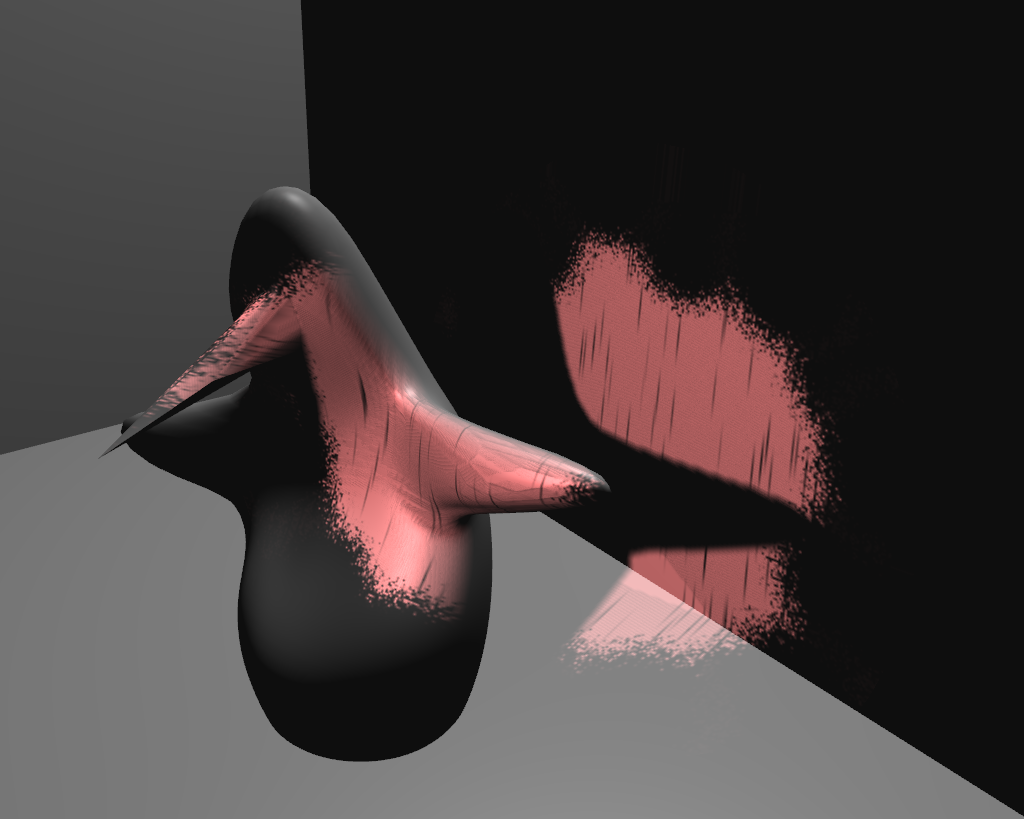
\includegraphics[width=1.8in]{../fancy_light_spot_shape}
  \caption{Światło filtrowane przez teksturę. Istotne jest że światło ciągle rzuca poprawny cień.}
\end{figure}
\end{frame}

\begin{frame}{Efekty tekstur}
Tekstury można modyfikować przy użyciu efektów. Tekstury mają mnóstwo
zastosowań (to po prostu macierz, zazwyczaj 2D lub 3D), więc wiele nowych
możliwości.
\end{frame}

\begin{frame}{Proceduralne tekstury na GPU}
Proceduralne tekstury to po prostu funkcje 2D lub 3D ->
kolor, wektor normalny, etc.

Tworzenie ich zawsze było łatwe, ale stare metody miały wadę:
ponieważ nie jest to tekstura dla renderera, znikają możliwości wygodnego
generowania i przypisywania współrzędnch. Rozwiązujemy to przez
\texttt{ShaderTexture}.

\begin{columns}[T]
  \begin{column}{1in}
    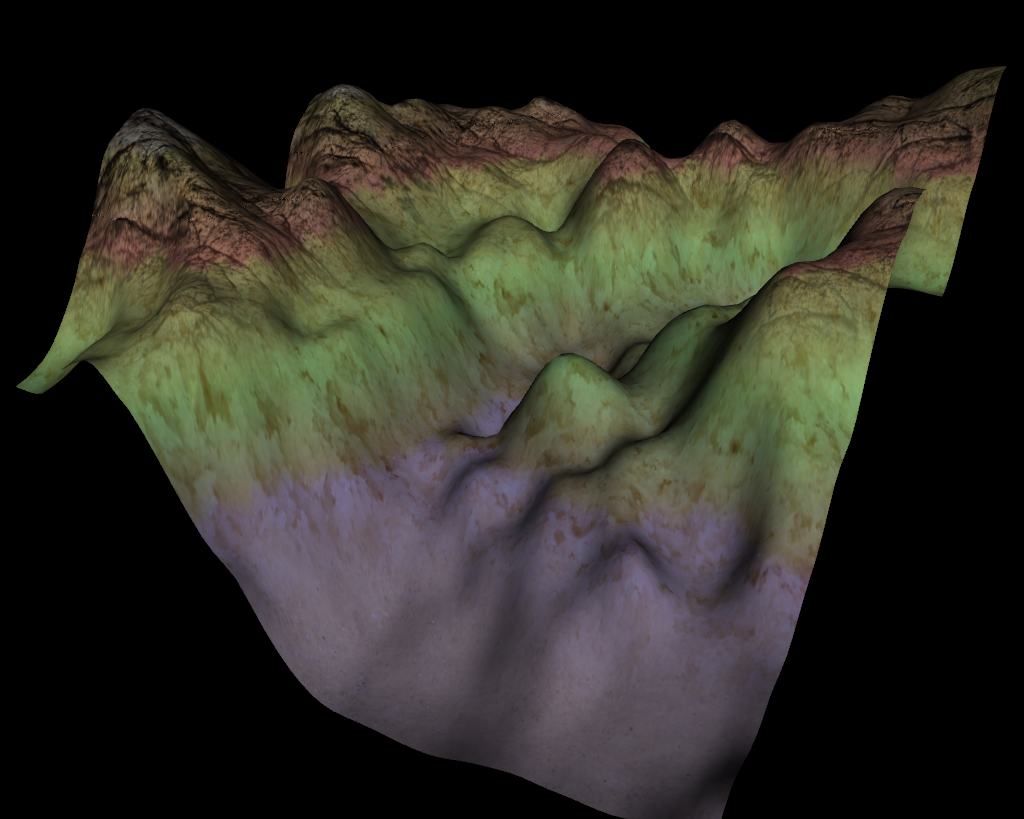
\includegraphics[width=1.5in]{../terrain}
  \end{column}
  \begin{column}{1in}
    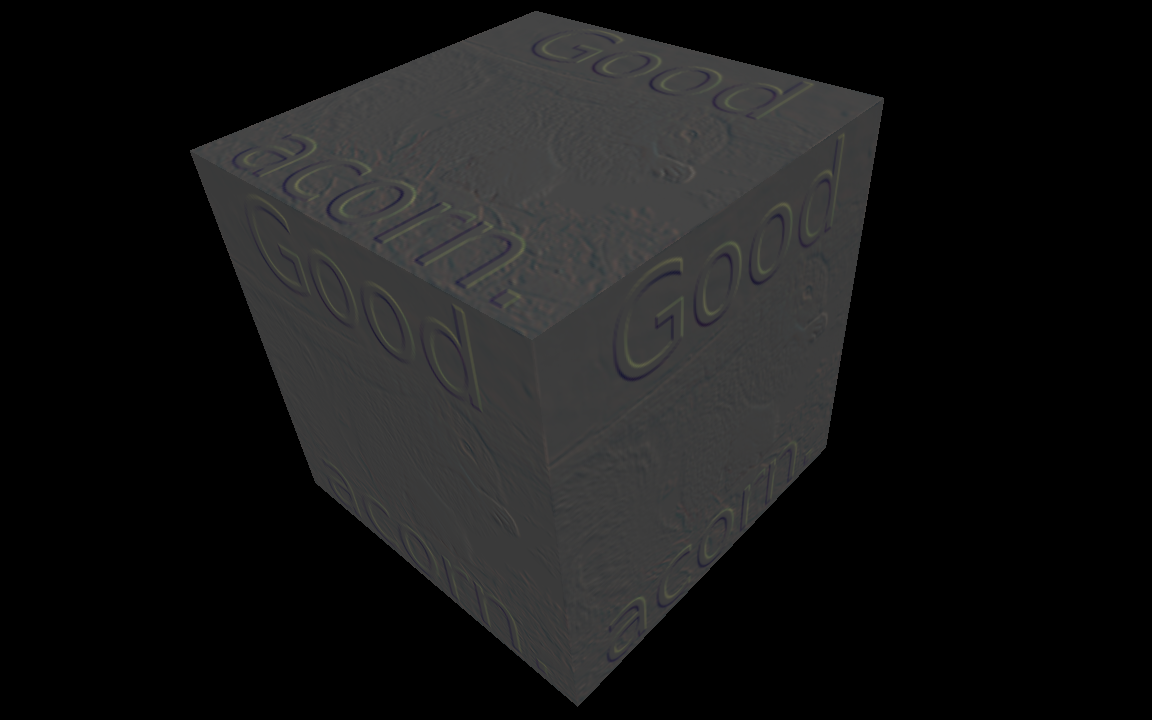
\includegraphics[width=1.5in]{../shader_texture_edge_detection}
  \end{column}
  \begin{column}{1in}
    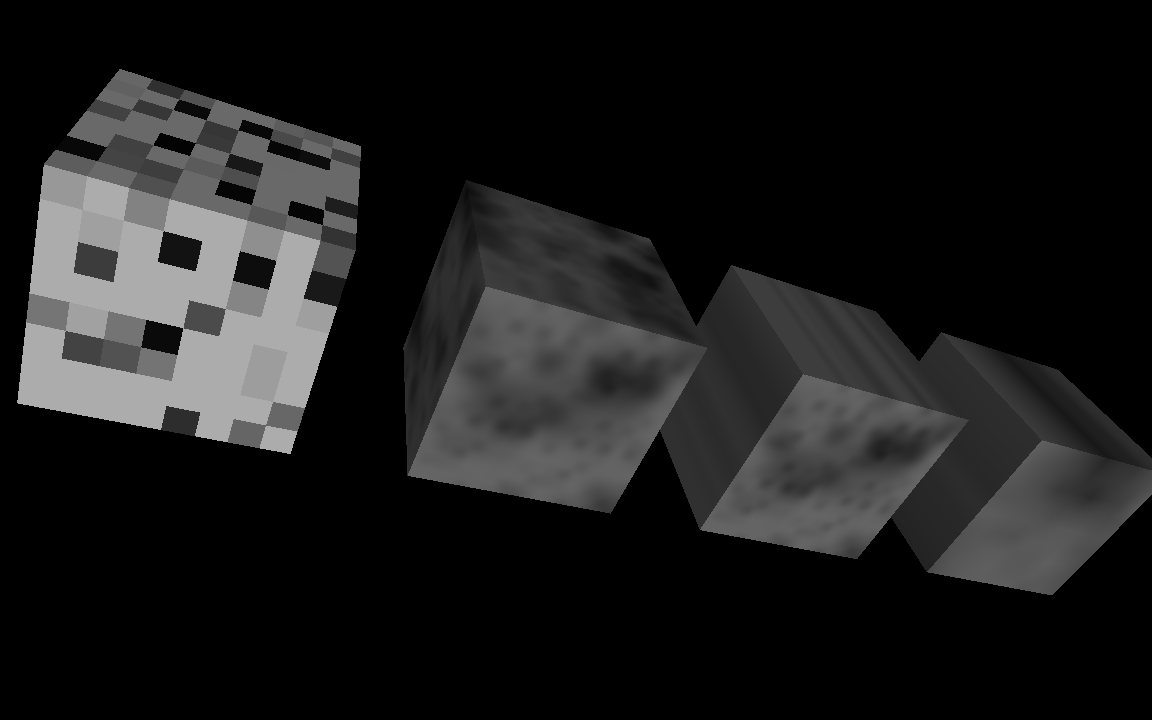
\includegraphics[width=1.5in]{../noise}
  \end{column}
\end{columns}

\end{frame}

\begin{frame}{Efekty działające na grupę}
Naturalne rozszerzenie. Przykładowo, ciekawa mgła.

\begin{figure}
  \centering
  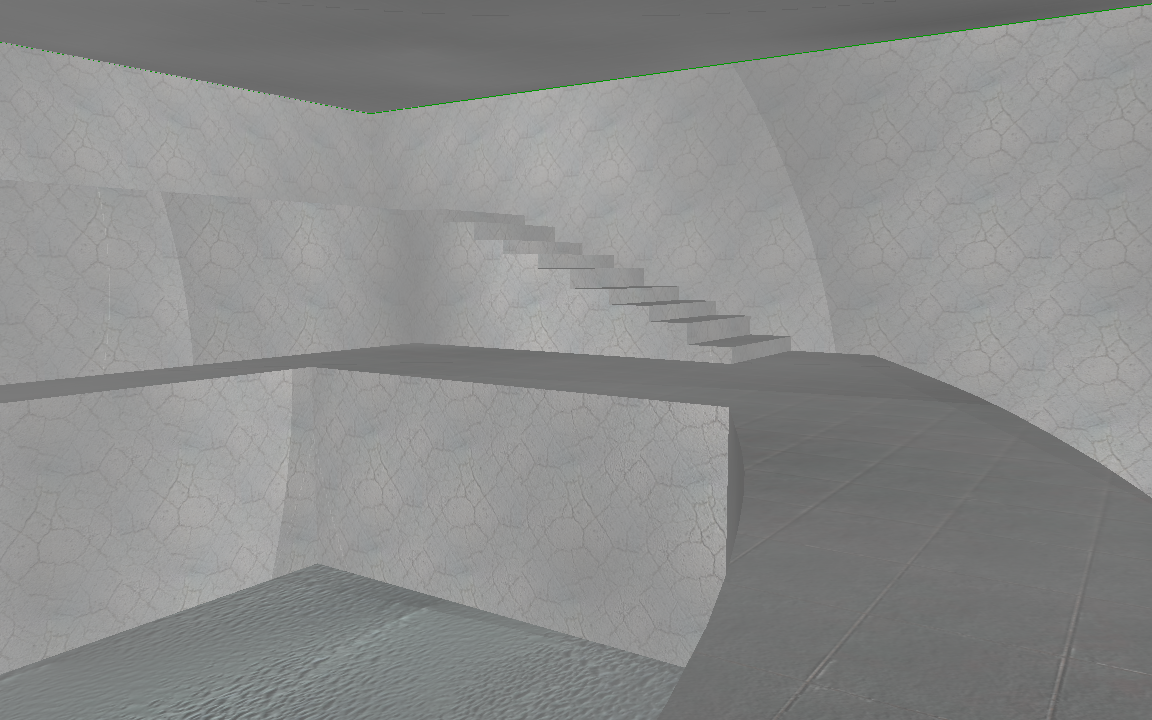
\includegraphics[width=1.8in]{../volumetric_animated_fog_all}
  \caption{Kłębiasta, ruchoma mgła (sauna).}
\end{figure}

(Kod: \texttt{demo\_models/compositing\_shaders/volumetric\_animated\_fog.x3dv}.\\
\textbf{Krótki i działa na dowolnym modelu 3D!}\\
Unline other implementation.)
% Turn on/off fog.

\end{frame}

\begin{frame}{Definiuj własne gniazda}
Twój efekt może definiować gniazda do użycia przez inne efekty.
Trywialne: magiczny komentarz \texttt{/* PLUG: ... */}.
\end{frame}

\begin{frame}{Przykłady na koniec}
Woda:

\begin{figure}
  \centering
  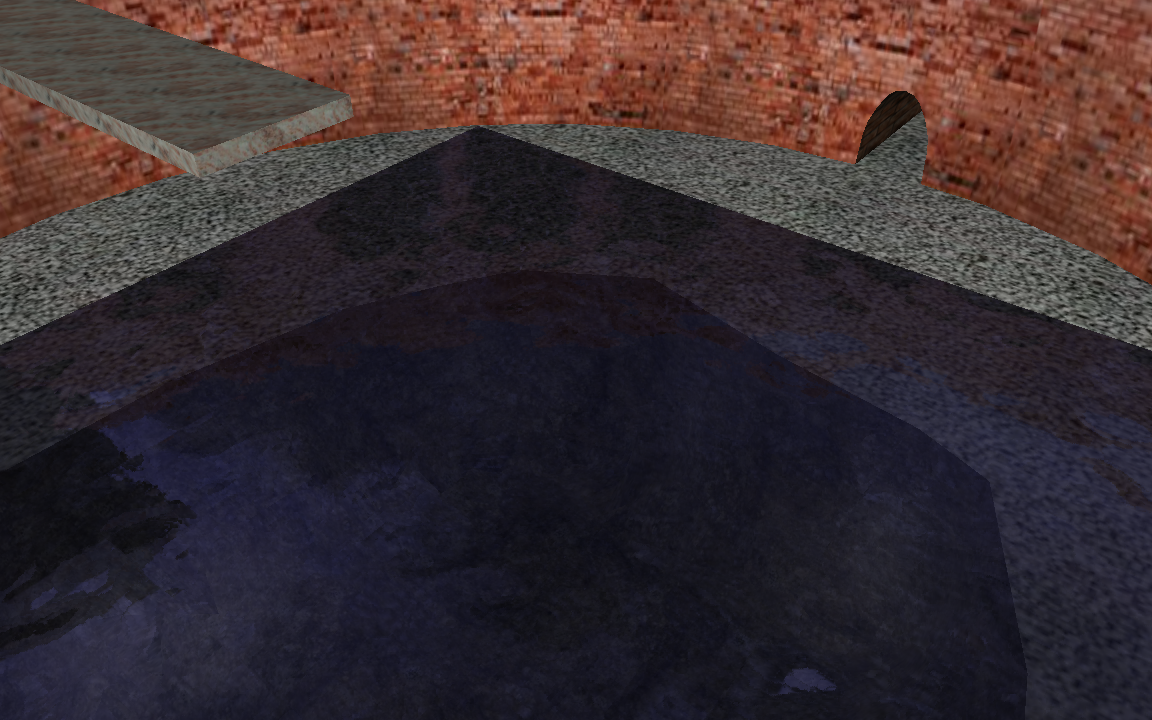
\includegraphics[width=1.8in]{../water_shaders_3}
  \caption{Woda, połączenie kilku efektów: generuj wektory normalne, transformuj je do eye space, połącz z reflection + refraction}
\end{figure}

Kwiatki:

\begin{figure}
  \centering
  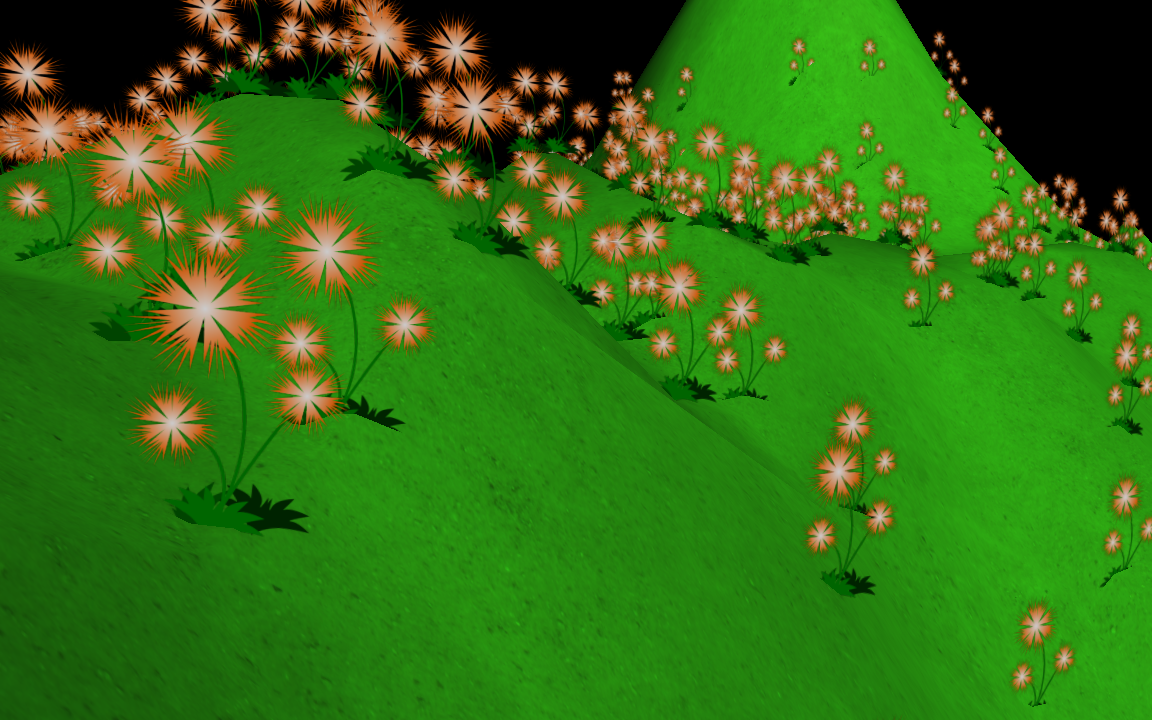
\includegraphics[width=1.8in]{../flowers}
  \caption{Kwiatki: transformacja zmieniana przez shader.}
\end{figure}
\end{frame}

\section{Pytania?}

\begin{frame}[t]

\begin{center}
{\small
Wszystko jest już zaimplementowane, open-source (LGPL), w moim silniku:\\
{\color{blue} \textbf{\texttt{http://vrmlengine.sourceforge.net/}}}\\
Instrukcje jak pobrać i oglądać przykładowe modele dotyczące komponowania
shaderów:\\
{\color{blue} \textbf{\texttt{http://vrmlengine.sourceforge.net/\\
compositing\_shaders.php}}}}
\end{center}

\vspace{0.25in}

\begin{center}
{\Large Dziękuję za uwagę!}
\end{center}

%\vspace{0.1in}

\begin{center}
{\Huge \alert{Pytania?}}
\end{center}

\end{frame}

\end{document}
